\documentclass[a4paper,12pt]{article}
\usepackage[a4paper, margin=2.5cm]{geometry}
\usepackage[pdftex]{graphicx}
\usepackage{tikz}
\usepackage{pgfplots}
\usepackage{enumitem}
\usepackage{float}
\usepackage[document]{ragged2e}
\usepackage[utf8]{inputenc}
\usepackage[T1]{fontenc}
\usepackage[spanish,es-tabla]{babel}
\renewcommand{\shorthandsspanish}{}
\usepackage{xurl}
\usepackage{lipsum}
\usepackage{mwe}
\usepackage{multicol}
\usepackage{siunitx}
\usepackage{listings}
\usepackage{circuitikz}
\usepackage{tabularray}

\graphicspath{ {/home/saikkopat/Documents/school/CE/P3/} }

\title{Práctica 3: Leyes de Kirchhoff}
\author{González Cárdenas Ángel Aquilez \and Sánchez González Daniel Iván}

\begin{document}

\begin{titlepage}
	\begin{tikzpicture}[overlay, remember picture]
		\path (current page.north east) ++(-0.3,-1.5) node[below left] {
\includegraphics[width=0.35\textwidth]{/home/saikkopat/Documents/LOGOS IPN/EscudoESCOM}};
	\end{tikzpicture}
	\begin{tikzpicture}[overlay, remember picture]
		\path (current page.north west) ++(1.5,-1) node[below right] {
\includegraphics[width=0.2\textwidth]{/home/saikkopat/Documents/LOGOS IPN/logo}};
	\end{tikzpicture}
	\begin{center}
		\vspace{-1.5cm}
		{\LARGE Instituto Politécnico Nacional\par}
		\vspace{.5cm}
		{\LARGE Escuela Superior de Cómputo\par}
		\vspace{.5cm}
		{\Large Laboratorio de Circuitos Eléctricos\par}
		\vspace{2cm}
		{\large Unidad de aprendizaje:}\\{\Large Circuitos Eléctricos\par}
		\vspace{2cm}
		{\scshape\Huge Práctica 3\par}
		{\itshape\Large Leyes de Kirchhoff\par}
		\vfill
		\vspace{.7cm}
		{\Large Grupo: 3CV2\par}
		\vspace{.7cm}
		{\Large Integrantes:\\González Cárdenas Ángel Aquilez\\Sánchez González Daniel Iván\par}
		\vspace{1cm}
		{\Large Profesor: Vázquez Ortíz Mijaíl\par}
		\vspace{1cm}
		{\large Fecha de realización: 26 de marzo de 2023\par}
		{\large Fecha de entrega: 03 de abril de 2023\par}
		\vfill
	\end{center}
\end{titlepage} 

\newpage

\tableofcontents

\newpage

\usepgfplotslibrary{units}

\section*{Objetivo}

\textbf{Objetivo}: El alumno aplicará las leyes de Ohm y las leyes de Kirchhoff para voltajes y corrientes, al análisis de circuitos eléctricos, para que al finalizar la práctica, esté en posibilidades de comprobar y corroborar los cálculos obtenidos por medio de técnicas y métodos ya establecidos, como son los siguientes:\par

\begin{itemize}
	\item Ley de Kirchhoff de voltaje, en una serie de mallas.
	\item Ley de Kirchhoff de corriente, en una serie de nodos.
\end{itemize}


El alumno utilizara los siguientes materiales y equipo:

\begin{multicols}{2}
\textbf{Equipo}\\
\begin{itemize}[nosep]
	\item 1 Multímetro digital
	\item 1 Fuente de voltaje variable de corriente directa
\end{itemize}

\columnbreak

\textbf{Material}\\
\begin{itemize}[nosep]
	\item 1 \textit{Protoboard}
	\item 2 Resistor de \SI{330}{\ohm} a $\frac{1}{2}$ de \si{\watt}
	\item 2 Resistor de \SI{470}{\ohm} a $\frac{1}{2}$ de \si{\watt}
	\item 2 Resistor de \SI{560}{\ohm} a $\frac{1}{2}$ de \si{\watt}
	\item 6 puntas banana-caimán
	\item 4 puntas caimán-caimán
	\item Alambres para conexiones
\end{itemize}

\end{multicols}

\section{Introducción teórica}

Nuestro desarrollo en las leyes de Kirchhoff no incluye pruebas rigurosas, solo se estudiará el contexto básico para el entendimiento de la teoría de circuitos.\\
Dos leyes básicas para el análisis de circuitos que contienen elementos de tipo resistivo, inductivo y capacitivo, son las postuladas por el físico alemán \emph{Gustav Robert Kirchhoff} (1824 – 1887) la “Ley de corriente de Kirchhoff (LCK)” y la “Ley de voltajes de Kirchhoff (LVK)”.

\vspace{.5cm}

La ley de corriente de Kirchhoff postula que:\\
\textit{	“La suma algebraica de las corrientes que inciden en un nodo son cero”}.\\

\vspace{.5cm}

La ley de Kirchhoff para voltajes postula que:\\
\textit{ “La suma algebraica de los voltajes alrededor de cualquier trayectoria cerrada en un circuito es cero en todo instante”}.\\

\vspace{.5cm}

Entendiéndose por cerrada, el recorrido a través de una serie de nodos que terminan en el nodo inicial sin pasar por ningún nodo más de una vez. Una trayectoria cerrada suele llamarse \emph{lazo} ó \emph{bucle}.

Por ejemplo, considere el circuito que se muestra en la Figura 2, es un circuito que consiste de dos trayectorias cerradas.\\

\newpage

\section{Desarrollo}

\subsection{Comprobación de la Ley de Kirchhoff para voltaje}

Sin encender las fuente de voltaje, se armó el circuito de la Figura 1 sobre el protoboard. Después, se procedió a ajustar el voltaje suministrado como se muestra en la Tabla 1. 

\vspace{0.5cm}

\begin{figure}[h!]
	\centering
	  \begin{circuitikz}[american, voltage dir=RP] 
	  		\draw	(0,0)
	  		to[battery, l=$\SI{9}{\volt}$, a=$V_{s1}$] (0,4)
	  		to[short, -*] node[anchor=south] {A}  (0,4)
	  		to[R, a=$R_1$, l=$\SI{470}{\ohm}$] (3,4)
	  		to[short, -*] node[anchor=south] {B} (3,4)
	  		to[battery, l=$\SI{5}{\volt}$,a=$V_{s2}$, invert] (6,4) 
	  		to[short, -*] node[anchor=south] {C} (6,4)
			to[R, a=$R_2$, l=$\SI{330}{\ohm}$] (9,4)
			to[short, -*] node[anchor=south] {D} (9,4)
			to[R, a=$R_3$, l=$\SI{560}{\ohm}$] (9,0) -- (4.5,0)
			to[short, -*] node[anchor=north] {0} 
			(4.5,0) -- (0,0);
		\end{circuitikz}
	\caption{Circuito 1}
\end{figure}

\vspace{1cm}

\begin{table}[ht!]
\setlength\tabcolsep{3pt}
\begin{center}
\begin{tblr}{|c c c c c c|}
	\hline
		Mediciones
		& \multicolumn{1}{|p{2cm}|}{\centering Valor \\ teórico}
		& \multicolumn{1}{|p{2cm}|}{\centering Valor \\ medido}
		&	\multicolumn{1}{|p{2cm}|}{\centering Potencia \\ teórica}
		& \multicolumn{1}{|p{2cm}|}{\centering Potencia \\ medida}
		& \multicolumn{1}{|p{2cm}|}{\centering Tipo de \\ potencia}
		\\ [0.5ex]	\hline
 Voltaje $V_{0A}$ & \SI{9}{\volt} & \SI{-8.99}{\volt} & \SI{26.46}{\mW} & \SI{26.43}{\mW} & S \\ \hline
 Voltaje $V_{AB}$ & \SI{1.38}{\volt} & \SI{3.99}{\volt} & \SI{4.05}{\mW} & \SI{11.73}{\mW} & A \\ \hline
 Voltaje $V_{BC}$ & \SI{5}{\volt} & \SI{5}{\volt} & \SI{14.7}{\mW} & \SI{14.7}{\mW} & S \\ \hline
 Voltaje $V_{CD}$ & \SI{971}{\mV} & \SI{0.123}{\mV} & \SI{2.85}{\mW} & \SI{361.6}{\nano \watt} & A \\ \hline
 Voltaje $V_{D0}$ & \SI{1.65}{\volt} & \SI{0.225}{\mV} & \SI{4.82}{\mW} & \SI{661.5}{\nano \watt} & A \\ \hline
 & $\sum = \SI{14}{\volt}$ & $\sum = \SI{0}{\volt}$ & $\sum = \SI{52.2}{\mW}$ & $\sum = \SI{52.86}{\mW}$ &  \\ \hline
 
\end{tblr}
\label{table:1}
\caption{Valores de voltaje teóricos y experimentales}
\end{center}
\end{table}

\newpage



\subsection{Comprobación de la Ley de Kirchhoff de corriente}

Sin encender las fuente de voltaje, se armó el circuito de la Figura 2 sobre el protoboard. Después, se procedió a ajustar el voltaje suministrado y conectar las fuentes de voltaje al circuito.

\vspace{0.5cm}

\begin{figure}[h!]
	\centering
	  \begin{circuitikz}[american, voltage dir=RP] 
	  		\draw	(0,0)
	  		to[battery, l=$\SI{9}{\volt}$, a=$V_{s1}$] (0,4)
	  		to[short, -*] node[anchor=south] {A}  (0,4)
	  		to[R, a=$R_1$, l=$\SI{470}{\ohm}$] (4,4)
	  		to[short, -*] node[anchor=south] {B} (4,4)
			to[R, a=$R_3$, l=$\SI{560}{\ohm}$] (8,4)
			to[short, -*] node[anchor=south] {C} (8,4)
			to[battery, l=$\SI{5}{\volt}$, a=$V_{s2}$, invert] (8,0) --(4,0)
			to[short, -*] node[anchor=north] {0} (4,0) -- (0,0);
			\draw (4,4)
			to[R, a=$R_2$, l=$\SI{330}{\ohm}$] (4,0);
		\end{circuitikz}
	\caption{Circuito 2}
\end{figure}

\vspace{1cm}

\begin{table}[h!]
\begin{center}
\begin{tabular}{|c c c|}
	\hline
Mediciones & Valor teórico & Valor medido  \\ [0.6ex]	\hline
Corriente $i_1$ (Rama izquierda) & \SI{10.54}{\mA} & \SI{10.681}{\mA} \\ \hline
Corriente $i_2$ (Rama central) & \SI{12.24}{\mA} & \SI{12.246}{\mA} \\ \hline
Corriente $i_3$ (Rama derecha) & \SI{1.70}{\mA} & \SI{1.774}{\mA} \\ \hline
 
\end{tabular}
\label{table:2}
\caption{Valores de corriente teóricos y experimentales}
\end{center}
\end{table}

\vspace{1cm}

\begin{table}[ht!]
\setlength\tabcolsep{3pt}
\begin{center}
\begin{tblr}{|c c c c c c|}
	\hline
		Mediciones
		& \multicolumn{1}{|p{2cm}|}{\centering Valor \\ teórico}
		& \multicolumn{1}{|p{2cm}|}{\centering Valor \\ medido}
		&	\multicolumn{1}{|p{2cm}|}{\centering Potencia \\ teórica}
		& \multicolumn{1}{|p{2cm}|}{\centering Potencia \\ medida}
		& \multicolumn{1}{|p{2cm}|}{\centering Tipo de \\ potencia}
		\\ [0.5ex]	\hline
 Voltaje $V_{0A}$ & \SI{9}{\volt} & \SI{8.997}{\volt} & \SI{94.8}{\mW} & \SI{92.07}{\mW} & S \\ \hline
 Voltaje $V_{AB}$ & \SI{4.95}{\volt} & \SI{4.975}{\volt} & \SI{52.17}{\mW} & \SI{50.89}{\mW} & A \\ \hline
 Voltaje $V_{B0}$ & \SI{4.039}{\volt} & \SI{4.021}{\volt} & \SI{49.43}{\mW} & \SI{49.24}{\mW} & A \\ \hline
 Voltaje $V_{BC}$ & \SI{0.95}{\volt} & \SI{-0.976}{\volt} & \SI{1.61}{\mW} & \SI{1.731}{\mW} & A \\ \hline
 Voltaje $V_{C0}$ & \SI{5}{\volt} & \SI{4.998}{\volt} & \SI{8.5}{\mW} & \SI{8.866}{\mW} & S \\ \hline
 & & & $\sum = \SI{206.15}{\mW}$ & $\sum = \SI{202.797}{\mW}$ &  \\ \hline
 
\end{tblr}
\label{table:3}
\caption{Valores de voltaje teóricos y experimentales}
\end{center}
\end{table}

\vspace{1cm}


\section{Cuestionario}

\vspace{1cm}

\begin{enumerate}

\item Defina que es un nodo en un circuito eléctrico.\\
Según Boylestad: \textit{Es la unión de dos o más ramas en una red}.
\item Defina que es un circuito eléctrico.\\
Es un conjunto de elementos pasivos y activos interconectados.
\item Exprese en forma matemática la Ley de Kirchhoff para corriente.\\
\[\sum i_{entrada} = \sum i_{salida}\]
\item Defina que es una trayectoria cerrada en un circuito eléctrico.\\
Un conjunto de elementos interconectados de principio a fin, es decir, sin que alguno de sus componentes no esté conectado al circuito.

\item Defina que es una caída de voltaje.\\
El cambio en la cantidad de voltaje de un elemento de un circuito, o bien, donde se consume voltaje.


\end{enumerate}


\newpage

\section{Conclusiones}

\vspace{.5cm}

{\Large González Cárdenas Ángel Aquilez}\\
\vspace{.3cm}
Con lo establecido por la ley de Ohm, y las leyes de corriente y voltaje de Kirchhoff, se calculó un resultado teórico para la corriente, voltaje y potencia en un circuito; comparando los valores calculados con los obtenidos de los instrumentos de  medición, se obtuvieron resultados similares para las mediciones de la LCK, diferenciándose en decimales, y con resultados diferentes para la LVK producto de la conexión de las fuentes.\par

\vspace{1cm}

{\Large Sánchez González Daniel Iván}\\
\vspace{.3cm}
Al termino de la práctica, se apreció cómo se comporta las leyes de Ohm y Kirchhoff (para voltajes y corrientes) en un circuito. Se encontró que para el Circuito 1, debido a la forma de conexión de las fuentes de voltaje, el circuito no suministró \SI{14}{\volt} sino \SI{4}{\volt} al resto del circuito. Para las mediciones de la LCK, los resultados calculados y medidos fueron similares.
\par

\section{Bibliografía}

\begin{itemize}
\item Boylestad, R. L., Salas, R. N., y Rizo, J. F. P. (2011). Introducción al análsis de circuitos. (página 131).
\end{itemize}

\section{Anexos}
\subsection{Simulaciones de los circuitos}

A continuación de presentan los resultados de las simulaciones de los circuitos de las figuras 1 y 2 para contrastarlos con las mediciones y cálculos realizados. Se generaron gracias a la aplicación multiplataforma \textit{EveryCircuit}\texttrademark. \\



\vspace{.5cm}

\begin{figure}[!h]
\centering
	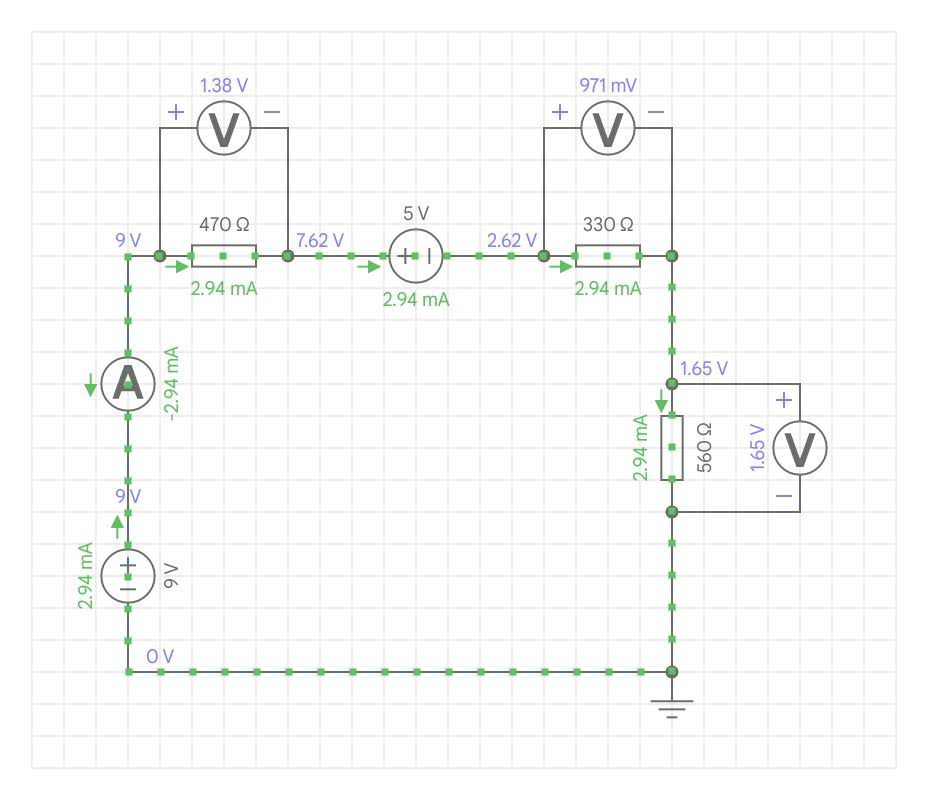
\includegraphics[width=.7\textwidth]{fig1}
	\label{fig5}
	 \caption{Simulación del Circuito 1}
\end{figure}

\vspace{.5cm}


\begin{figure}[!h]
\centering
	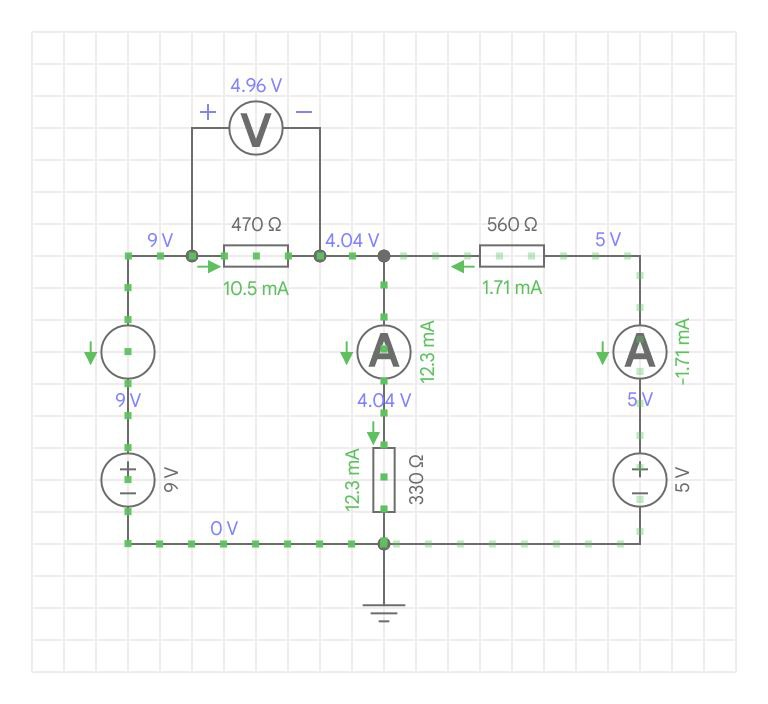
\includegraphics[width=.7\textwidth]{fig2}
	\label{fig5}
	 \caption{Simulaciones del circuito 2}
\end{figure}

\vspace{.5cm}

\end{document}